\documentclass[conference]{IEEEtran}
\IEEEoverridecommandlockouts

% --- requested packages ---
\usepackage{graphicx}
\usepackage{amsmath}
\usepackage{booktabs}
\usepackage{hyperref}
\usepackage{multirow}
\usepackage{xcolor}
% encoding safety (not in the requested list, added so pdflatex handles any
% stray unicode; all special symbols below are also written as LaTeX macros)
\usepackage[utf8]{inputenc}
\usepackage[T1]{fontenc}

\graphicspath{{figures/}}

\begin{document}

\title{AgentLens: Behavioral Trajectory Learning for
Automated Tool Selection in AI-Assisted Cybersecurity Agents}

\author{
\IEEEauthorblockN{Kranthi Gadi, Ricardo Calix}
\IEEEauthorblockA{Purdue University Northwest\\
Hammond, IN, USA\\
\{kbitra, rcalix\}@pnw.edu}
}

\maketitle

% ---------------------------------------------------------------- ABSTRACT
\begin{abstract}
Large language model (LLM) agents increasingly orchestrate external tools to
complete multi-step tasks, but on ambiguous or long-horizon queries they select
tools inconsistently, latching onto surface keywords rather than task intent. We
present \textbf{AgentLens}, a framework that treats an agent's own tool
decisions as training data: a logging wrapper records \emph{(prompt, tool)}
behavioral trajectories as the agent runs, and a lightweight classifier learns a
tool-selection policy that replaces LLM routing. We instantiate AgentLens on a
cybersecurity attacker/defender scenario with 11 SSH-based tools and a 640-query
labeled dataset spanning direct and deliberately ambiguous queries. A TF-IDF $+$
SVM policy, evaluated with 5-fold cross-validation, reaches
\textbf{98.3\% $\pm$ 0.8\%} accuracy versus \textbf{79.4\%} for the Llama 3.2 3B
baseline, and \textbf{94.5\% $\pm$ 2.5\%} versus \textbf{73.5\%} on hard queries,
while routing each query in \textbf{0.3 ms} versus \textbf{209 ms}
($700\times$ faster). Trained trajectory policies can thus replace LLM tool
routing---faster, cheaper, and more accurate.
\end{abstract}

\begin{IEEEkeywords}
tool selection, LLM agents, behavioral cloning, cybersecurity, policy learning,
trajectory data
\end{IEEEkeywords}

% ---------------------------------------------------------------- INTRO
\section{Introduction}

Modern AI agents built on LLMs solve complex tasks by decomposing them into
steps and invoking external tools---search engines, code interpreters, shell
commands. The quality of such an agent depends less on its language fluency than
on a narrower competence: given the current task, \emph{which tool should it
call?} On clearly worded requests this is easy. On ambiguous, underspecified, or
multi-step requests it is not, and small locally-hosted models are especially
brittle. They tend to match a salient keyword in the prompt to a tool name and
ignore the surrounding intent---reading ``scan the target and see what comes
back'' as a version scan when a port sweep was meant.

This failure is costly in cybersecurity. An AI-assisted penetration-testing
agent that chooses the wrong reconnaissance tool wastes time and, worse, can
miss an exposed service and the vulnerability behind it. A defensive agent that
reads the wrong log misses an active intrusion. As agents are given real
offensive and defensive tooling, reliable tool selection becomes a safety
property, not a convenience.

Rather than fine-tuning the LLM---expensive, opaque, and hard to reproduce on
commodity hardware---AgentLens takes a behavioral view. As the agent runs, every
tool decision it makes is logged as a \emph{(prompt, tool)} pair. These
trajectories become a labeled dataset from which a lightweight classifier learns
the tool-selection policy directly. At inference the trained policy replaces the
LLM for routing: it is deterministic, sub-millisecond, and---because it is
trained on ground-truth labels rather than the LLM's own guesses---more accurate
than the model it replaces.

We instantiate and evaluate AgentLens on a cybersecurity attacker/defender
scenario. Our contributions are:

\begin{enumerate}
\item \textbf{A trajectory-collection framework} that automatically and
transparently logs an agent's tool decisions with rich metadata, at zero
modeling cost.
\item \textbf{A labeled dataset} of 640 cybersecurity agent queries across 11
tools and three agent roles, with difficulty and query-style annotations that
isolate \emph{why} tool selection is hard.
\item \textbf{A trained policy classifier} that outperforms LLM routing by
\textbf{19 percentage points overall} and \textbf{21 points on ambiguous
queries}, at \textbf{$700\times$ lower latency}.
\item \textbf{An empirical analysis of LLM tool-selection failure modes},
showing that genuinely ambiguous and multi-step queries---not merely long
ones---are where a small LLM breaks down, and that a trained policy closes
exactly this gap.
\end{enumerate}

% ---------------------------------------------------------------- RELATED
\section{Related Work}

\textbf{LLM tool use.} Toolformer~\cite{toolformer} teaches a model to
self-annotate when to call APIs; ToolLLM~\cite{toolllm} and
Gorilla~\cite{gorilla} scale tool repertoires to thousands of APIs;
ReAct~\cite{react} interleaves reasoning traces with tool actions. These works
make the \emph{LLM itself} the router at every step. AgentLens instead
\emph{observes} the router and distills its task into a standalone classifier,
removing the LLM from the inference path entirely.

\textbf{AI agents in cybersecurity.} A growing line of work applies LLM agents
to automated penetration testing and vulnerability discovery, wiring models to
scanners and shells. This research focuses on \emph{what the agent can
accomplish}; AgentLens focuses on the reliability and cost of the tool-routing
decision underneath, and contributes a labeled benchmark for it in the security
domain.

\textbf{Behavioral cloning and imitation learning.} Learning a policy from
logged expert state--action pairs is the classical behavioral-cloning
setup~\cite{pomerleau1991}.
AgentLens is behavioral cloning where the ``state'' is a natural-language prompt
and the ``action'' is a tool; unlike typical imitation learning we clone against
\emph{corrected} ground-truth labels rather than the demonstrator's raw actions,
which lets the student exceed the teacher.

\textbf{Lightweight classifiers vs.\ LLMs for routing.} Recent systems use small
models or embeddings to route queries to models or tools for efficiency. We push
this to its conclusion for the tool-selection subproblem: a TF-IDF $+$ linear
model routes in 0.3 ms and, on our task, is more accurate than a 3B LLM.
AgentLens adds a difficulty-annotated benchmark that quantifies \emph{when} the
cheap router is enough and characterizes the LLM failure modes it repairs.

% ---------------------------------------------------------------- METHOD
\section{Methodology}

\subsection{System Architecture}

AgentLens has three components: the \textbf{agent}, the \textbf{trajectory
logger}, and the \textbf{policy classifier}. During data collection the agent
runs normally and the logger records every decision; after training, the policy
classifier can serve tool-routing decisions with no LLM in the loop.
Figure~\ref{fig:arch} shows this pipeline. The design keeps collection,
training, and inference in separate modules so the trained policy can be dropped
in front of, or in place of, the LLM router.

\begin{figure*}[!t]
\centering
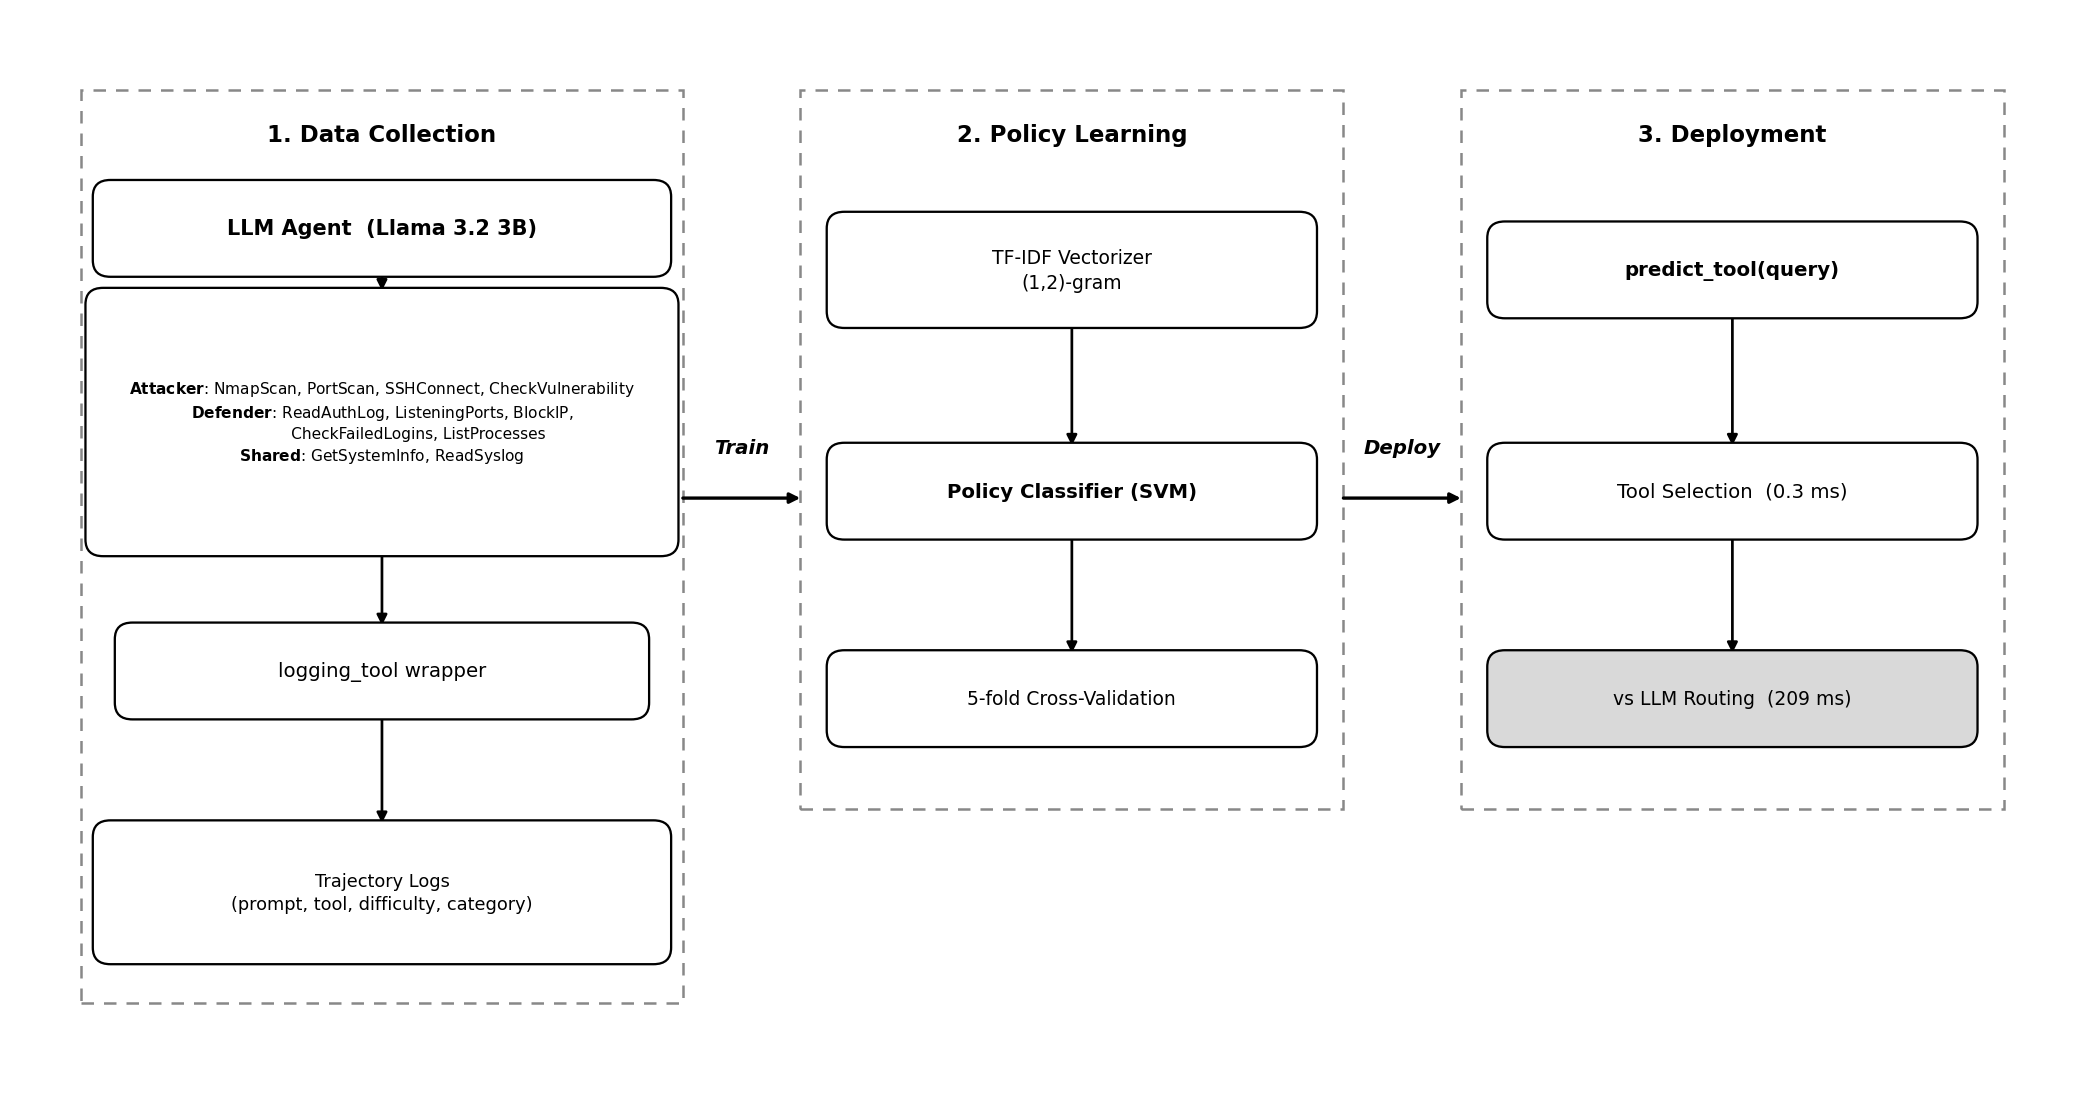
\includegraphics[width=\textwidth]{fig1_architecture}
\caption{AgentLens system architecture. Data collection logs the agent's
\emph{(prompt, tool)} decisions; policy learning trains a classifier on the
ground-truth labels; deployment routes future queries with the trained policy in
place of the LLM.}
\label{fig:arch}
\end{figure*}

\subsection{Trajectory Collection}

Every tool is wrapped by a \texttt{logging\_tool} decorator that appends a
trajectory record to a shared log before the tool executes; the wrapper is
transparent to the tool's return value, so collection adds no behavioral
overhead. Each record carries the schema \texttt{prompt}, \texttt{tool\_predicted},
\texttt{tool\_ground\_truth}, \texttt{agent\_role}, \texttt{difficulty},
\texttt{category}, \texttt{run\_id}. Crucially we log both the tool the LLM
\emph{chose} (\texttt{tool\_predicted}, the baseline) and the \emph{correct} tool
(\texttt{tool\_ground\_truth}, the training label); training on the latter is
what allows the policy to surpass the LLM.

We drive tool selection by calling the Ollama API directly rather than through a
CrewAI ReAct loop. The 3B model could not reliably emit CrewAI's verbose
tool-call format and frequently returned empty responses; a direct call asking
for a single-word tool name from the role's tool set is robust and also yields
cleaner trajectories (the original natural-language query is logged, not an
LLM-rewritten tool input). The LLM is \textbf{Llama 3.2 3B}~\cite{llama} served
locally by Ollama (\texttt{temperature=0}, \texttt{seed=42}).

\subsection{Dataset}

The cybersecurity scenario defines \textbf{11 tools} across three roles: an
\textbf{attacker} (4 tools: SSHConnect, NmapScan, PortScan, CheckVulnerability),
a \textbf{defender} (5 tools: ReadAuthLog, ListeningPorts, BlockIP,
CheckFailedLogins, ListProcesses), and \textbf{shared} utilities (2 tools:
GetSystemInfo, ReadSyslog). Tools are executed over SSH using the Paramiko
library~\cite{paramiko}. The dataset contains \textbf{640 labeled queries}
(attacker 261, defender 273, shared 106), generated by a seeded, reproducible
template expander. Each query is tagged \texttt{easy} (440, one unambiguous tool
cue) or \texttt{hard} (200), and hard queries are split into five style
categories designed to probe distinct failure modes (Table~\ref{tab:categories}).

\begin{table}[htbp]
\caption{Query Categories and LLM Accuracy (Llama 3.2 3B)}
\label{tab:categories}
\centering
\begin{tabular}{lrr}
\toprule
Category & $n$ & LLM Accuracy \\
\midrule
direct     & 440 & 82.0\% \\
ambiguous  & 40  & 57.5\% \\
multistep  & 40  & 70.0\% \\
trick      & 40  & 72.5\% \\
natural    & 40  & 82.5\% \\
opposite   & 40  & 85.0\% \\
\bottomrule
\end{tabular}
\end{table}

\subsection{Policy Classifier}

Queries are vectorized with \textbf{TF-IDF, (1,2)-grams,
\texttt{max\_features=5000}}. We train four classifiers---Logistic Regression,
linear SVM, MLP (64, 32), and Random Forest (100 trees)---on
\texttt{tool\_ground\_truth} using scikit-learn~\cite{sklearn}. We evaluate with
\textbf{5-fold StratifiedKFold} stratified on the combined
\texttt{tool}~$\times$~\texttt{difficulty} label, so every (tool, difficulty)
cell appears in each fold. The vectorizer is refit inside each fold to prevent
train/test leakage. We report mean $\pm$ standard deviation of overall accuracy,
hard-subset accuracy, and macro-F1 across folds.

% ---------------------------------------------------------------- RESULTS
\section{Experiments and Results}

\subsection{Main Results}

All four classifiers beat the LLM decisively (Table~\ref{tab:results}). The best,
linear SVM, improves on the LLM by \textbf{18.9 points overall} and
\textbf{21.0 points on hard queries}. The four models are statistically
indistinguishable overall (overlapping $\pm$ intervals); Random Forest has the
widest hard-query spread ($\pm$4.9\%). Figure~\ref{fig:confusion} is the
aggregated out-of-fold confusion matrix ($n = 640$, pooled 98.3\%): the 11
residual errors all fall between semantically adjacent
tools---NmapScan$\leftrightarrow$PortScan,
ListProcesses$\leftrightarrow$ListeningPorts, and within the log family
(ReadAuthLog, CheckFailedLogins, ReadSyslog).

\begin{table}[htbp]
\caption{Tool-Selection Accuracy and Latency (5-fold CV, mean $\pm$ std)}
\label{tab:results}
\centering
\begin{tabular}{lccc}
\toprule
Method & Overall Acc & Hard Acc & Latency \\
\midrule
LLM Baseline    & 79.4\%                  & 73.5\%                  & 209 ms \\
\textbf{SVM}    & \textbf{98.3\% $\pm$ 0.8\%} & \textbf{94.5\% $\pm$ 2.5\%} & 0.3 ms \\
LogReg          & 98.1\% $\pm$ 0.6\%      & 94.0\% $\pm$ 2.0\%      & 0.3 ms \\
MLP             & 98.0\% $\pm$ 0.8\%      & 93.5\% $\pm$ 2.5\%      & 0.3 ms \\
RF              & 97.8\% $\pm$ 1.5\%      & 93.0\% $\pm$ 4.9\%      & 0.3 ms \\
\bottomrule
\end{tabular}
\end{table}

\begin{figure*}[!t]
\centering
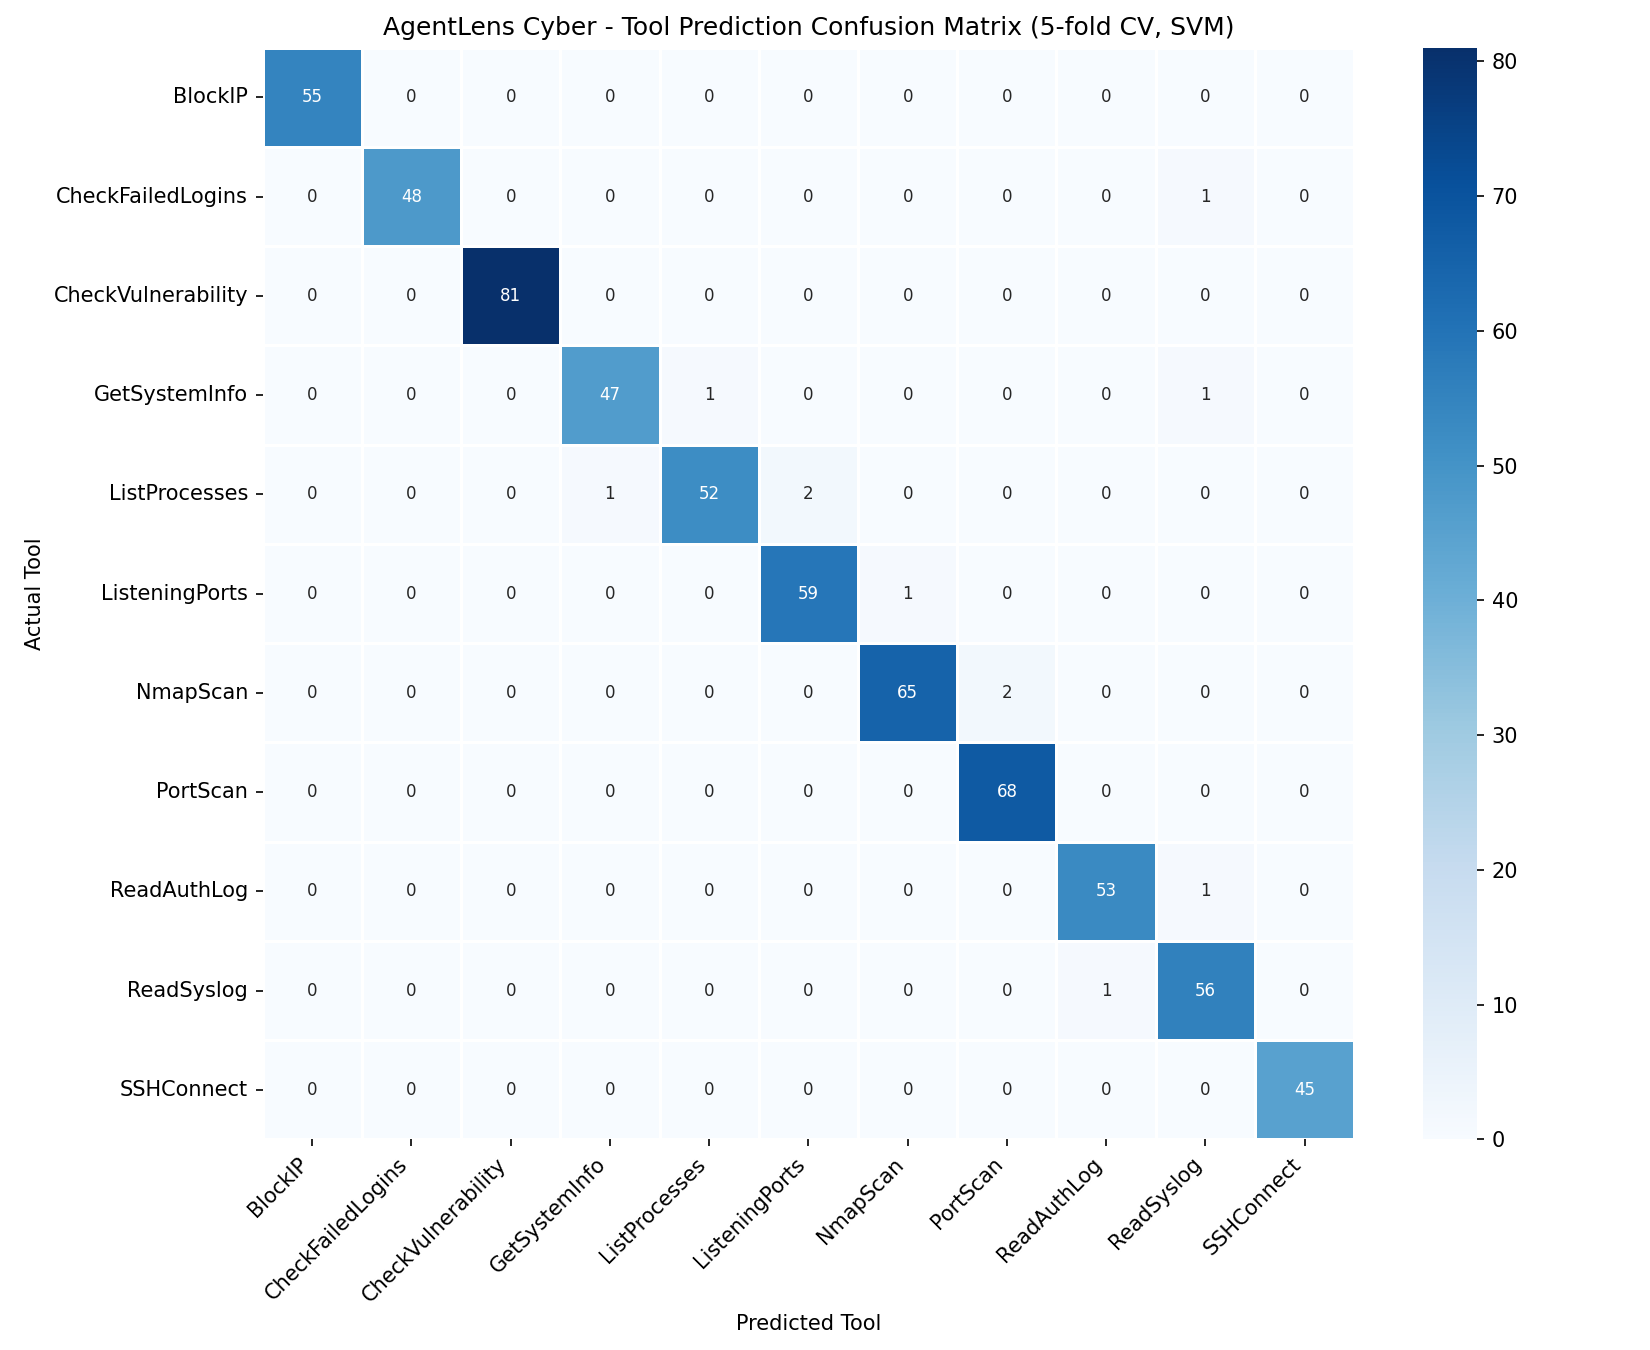
\includegraphics[width=0.82\textwidth]{fig2_confusion_matrix}
\caption{Aggregated out-of-fold confusion matrix (5-fold CV, best SVM model,
$n=640$, pooled 98.3\%). The 11 residual errors fall between semantically
adjacent tools.}
\label{fig:confusion}
\end{figure*}

\subsection{LLM Failure-Mode Analysis}

The category breakdown (Table~\ref{tab:categories}, Fig.~\ref{fig:category})
localizes where the LLM fails. Accuracy collapses on \textbf{ambiguous} queries
(57.5\%) and is weak on \textbf{multistep} (70.0\%) and \textbf{trick} (72.5\%)
queries, while remaining high on direct, natural, and opposite phrasings. The
dominant confusion is NmapScan vs.\ PortScan: asked to ``scan the target and see
what comes back,'' the 3B model cannot decide between a service/version scan and
a port sweep because neither keyword is present. In short, the model latches onto
surface keywords and, when they are absent or misleading, guesses. The trained
classifier does not share this weakness: having learned from ground-truth labels
rather than the LLM's predictions, it recovers the intended tool on exactly these
categories, lifting hard-query accuracy from 73.5\% to 94.5\%.

\begin{figure}[htbp]
\centering
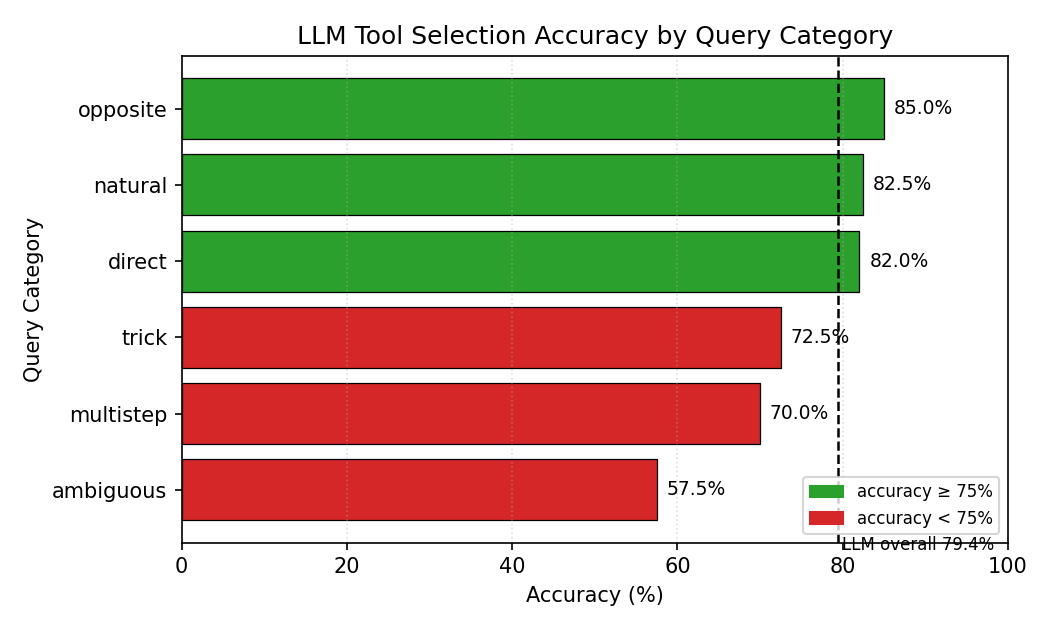
\includegraphics[width=\columnwidth]{fig3_category_accuracy}
\caption{LLM tool-selection accuracy by query category. Bars below the 75\%
threshold are the hard categories; the dashed line marks the 79.4\% overall LLM
baseline.}
\label{fig:category}
\end{figure}

\subsection{Latency Analysis}

Measured over real inference calls, the classifier routes a query in
\textbf{0.3 ms}; the LLM's median is \textbf{209 ms} and its mean \textbf{816
ms}, inflated by cold-start outliers (max 7.7 s). At the median this is a
$\sim$$700\times$ speedup (Fig.~\ref{fig:latency}); routing the full 640-query
set takes the classifier $\sim$0.2 s versus $\sim$135 s for the LLM.
Sub-millisecond, deterministic routing makes production deployment of the trained
policy feasible at scale, and removes per-query model cost entirely.

\begin{figure}[htbp]
\centering
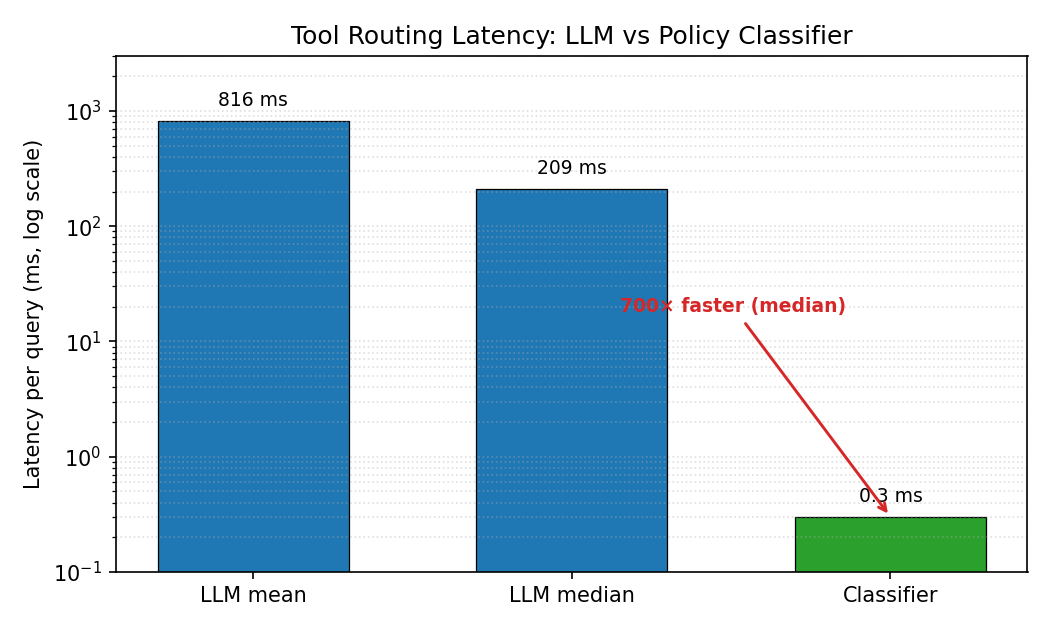
\includegraphics[width=\columnwidth]{fig4_latency}
\caption{Tool-routing latency (log scale): the policy classifier routes in
0.3 ms versus the LLM's 209 ms median, roughly $700\times$ faster.}
\label{fig:latency}
\end{figure}

% ---------------------------------------------------------------- DISCUSSION
\section{Discussion}

The results support a simple claim with broad implications for agentic AI: for
the bounded subproblem of tool selection, a policy \emph{cloned} from an agent's
own behavior---and corrected against ground truth---can be faster, cheaper, and
more accurate than the LLM that generated it. Where the general-domain version of
this task saturates (a linear model reaches $\sim$100\% because keywords fully
determine the tool), the cybersecurity task is genuinely hard, and the
$\sim$21-point hard-query gap is where the contribution lives.

\textbf{Limitations.} The dataset is synthetic, built from seeded templates
rather than real penetration-test transcripts, so absolute numbers may not
transfer to operator-written queries. Tool \emph{execution} is currently mocked
(canned outputs); tool \emph{selection} is real. And the baseline is a single 3B
model---larger LLMs may route better, narrowing the gap.

\textbf{Future work.} We are building isolated Linux VMs for real SSH tool
execution, so trajectories carry genuine tool outputs and success signals. We
will extend to a two-agent attacker/defender setup with reinforcement learning
(the journal follow-up), and evaluate a middle tier---fine-tuned small encoders
(BERT/Qwen via TRL)---between the TF-IDF policy and the full LLM.

% ---------------------------------------------------------------- CONCLUSION
\section{Conclusion}

We presented AgentLens, a framework that turns an LLM agent's own tool decisions
into training data for a lightweight tool-selection policy. On a cybersecurity
attacker/defender scenario with 11 tools and a 640-query difficulty-annotated
dataset, a TF-IDF $+$ SVM policy trained on collected trajectories reaches
98.3\% $\pm$ 0.8\% accuracy---19 points above the Llama 3.2 3B router it
replaces---and 94.5\% $\pm$ 2.5\% on hard, ambiguous queries where the LLM
manages only 73.5\%, all at 0.3 ms per query versus 209 ms. The key insight is
that the LLM generates its own training data for free, and that training against
ground-truth labels lets the student surpass the teacher precisely on the
ambiguous cases that matter. We will release the framework, dataset, and models
as open source. AgentLens lays the groundwork for a reinforcement-learning-based
multi-agent extension with real tool execution.

% ---------------------------------------------------------------- REFERENCES
\begin{thebibliography}{8}

\bibitem{toolformer}
T.~Schick \emph{et al.}, ``Toolformer: Language Models Can Teach Themselves to
Use Tools,'' in \emph{Advances in Neural Information Processing Systems
(NeurIPS)}, 2023.

\bibitem{toolllm}
Y.~Qin \emph{et al.}, ``ToolLLM: Facilitating Large Language Models to Master
16000+ Real-world APIs,'' in \emph{Int. Conf. on Learning Representations
(ICLR)}, 2024.

\bibitem{gorilla}
S.~G. Patil \emph{et al.}, ``Gorilla: Large Language Model Connected with Massive
APIs,'' in \emph{Advances in Neural Information Processing Systems (NeurIPS)},
2023.

\bibitem{react}
S.~Yao \emph{et al.}, ``ReAct: Synergizing Reasoning and Acting in Language
Models,'' in \emph{Int. Conf. on Learning Representations (ICLR)}, 2023.

\bibitem{llama}
Meta AI, ``Llama 3.2: Lightweight Models,'' 2024. [Online]. Available:
\url{https://ai.meta.com/blog/llama-3-2/}

\bibitem{sklearn}
F.~Pedregosa \emph{et al.}, ``Scikit-learn: Machine Learning in Python,''
\emph{Journal of Machine Learning Research}, vol.~12, pp.~2825--2830, 2011.

\bibitem{paramiko}
J.~Forcier \emph{et al.}, ``Paramiko: A Python Implementation of SSHv2,'' 2024.
[Online]. Available: \url{https://www.paramiko.org/}

\bibitem{pomerleau1991}
D.~Pomerleau, ``Efficient Training of Artificial Neural Networks for Autonomous
Navigation,'' \emph{Neural Computation}, vol.~3, no.~1, pp.~88--97, 1991.

\end{thebibliography}

\end{document}
